\subsection{Introduction}
One of the greatest challenges to global atmospheric modeling is representing the enormous range of physically relevant spatial scales given present day limits in high performance computing. For whatever the social, economic or political reasons may be, there is a persistent societal force on technological innovation that, has in the past, and will likely continue to result in increased computing power with time. The global atmospheric modeling community exploits advances in high performance computing as an opportunity to develop models that push the limits on the range of explicitly resolved scales, while maintaining reasonable computational throughput.

State-of-the-art General Circulation Models (GCMs) currently run at horizontal resolutions of approximately 100 km to 200 km, with high-resolution configurations of about 25 km to 50 km. A standard measure of model performance in the computational fluid dynamics community is that the numerical solution of a model converges with decreasing grid spacing. As discussed in \cite{W2008TELLUS}, convergence of the resolved fluid dynamical core is often satisfied in dry idealized test cases, but convergence of the moist GCM, including coupling with column physics, receives less attention. With the recent interest in variable resolution grids, and with horizontal resolutions approaching non-hydrostatic scales, there is increased awareness in the global atmospheric modeling community to develop GCMs with convergent solutions.

The Community Atmosphere Model (CAM), a GCM supported by the National Center for Atmospheric Research and the Department of Energy, has a long history of non-convergence \citep{KW1991JGR,WETAL1995CD,W1999T,W2008TELLUS,LETAL2011TELLUS,RJ2011MWR,RETAL2012ASL,OETAL2013JCLIM,RETAL2013JCLIM,ZetAl2014JCb,LETAL2015JCLIM}. Non-convergence is strong when CAM is coupled with version 4 physics and earlier, but there are indications of non-convergence when coupled with version 5 physics \citep{RETAL2012ASL,RM2016GRL}, although not as strong \citep{OETAL2013JCLIM,ZetAl2014JCb}. Many studies have found a strong sensitivity of large-scale simulation statistics to horizontal resolution, such as global cloud coverage, precipitation, surface pressure, vertical velocity and Hadley Cell strength \citep{KW1991JGR,WETAL1995CD,W2008TELLUS,LETAL2011TELLUS,RETAL2013JCLIM,OETAL2013JCLIM,ZetAl2014JCb} and more recently, the location of the eddy-driven jet \citep{LETAL2015JCLIM}. Although intuitively we may expect some of the variations in these large-scale statistics to be related, these studies have not made clear what relationship occurs in the simulations. 

Here, we study the sensitivity of CAM to horizontal resolution in an aqua-planet configuration, identify relationships between non-converging large-scale statistics using energy and moisture budgets and propose a possible explanation for the resolution sensitivity of the mean state. Other studies have focused on the convergence of CAM with respect to statistical extremes, such as precipitation extremes \citep{W2008TELLUS,LETAL2011TELLUS,YETAL2014JCLIM,OETAL2016JAMES} or tropical cyclones \citep{RJ2011JAMES}. Although the causes of non-convergence of mean and extreme statistics may be related, we primarily focus on the mean state in this study.

The non-convergence of CAM with increasing horizontal resolution has been attributed to the representation of moist processes \citep{W1999T,W2008TELLUS,OETAL2013JCLIM}. Studies on the convergence of CAM with respect to the model time-step have come to similar conclusions \citep{WO2003QJR,W2008TELLUS,W2013QJRMS,WETAL2015JAMES}. \cite{W2013QJRMS} argues that since convective adjustment in CAM versions 4 and earlier is limited by fixed relaxation timescales in the closure assumptions, a greater proportion of super-saturated air remains in a grid column as the time-step is reduced. Due to the sequential coupling of the moist physics, any super-saturated air remaining after the convection scheme has been called upon is condensed locally by the cloud macrophysics scheme, resulting in an increasingly buoyant state passed to the dynamical core as the time-step is reduced. Although the inconsistency of using fixed relaxation time-scales in the convection scheme is problematic, others have shown that the strong sensitivity of CAM to horizontal resolution remains when the time-step is held fixed \citep{W2008TELLUS,OETAL2013JCLIM,RETAL2013JCLIM} or the convection scheme is completely turned off \citep{OETAL2013JCLIM}. 

It has been recognized that the resolved vertical motion is participating in the sensitivity of precipitation extremes to resolution in CAM \citep{LETAL2011TELLUS,YETAL2014JCLIM}. \cite{RETAL2016CD} apply the mass continuity equation to the spectral properties of the horizontal wind in a suite of regional models to argue that resolved vertical velocity is expected to increase with resolution. The authors go on to formulate a heuristic scaling that linearly relates the resolved mass fluxes at cloud base to the precipitation rate in models, providing an explanation for the sensitivity of precipitation extremes to resolution. \cite{OETAL2016JAMES} show that the relationship of \cite{RETAL2016CD} provides an excellent fit to the precipitation rates in CAM. While the insights provided in \cite{RETAL2016CD} are valuable, there is no simple explanation for the spectral slope of the horizontal wind that can inform us on what processes are responsible for the increase in resolved vertical velocity with resolution in the models.

Here we analyze the dominant balances in the large-scale circulation’s response to varying horizontal resolution, and propose a possible explanation for the sensitivity of CAM to horizontal resolution at hydrostatic scales. We hypothesize that an increase in horizontal resolution leads to a reduction in horizontal scale of the diabatic forcing arising from the column physics, facilitating fine scale flow and faster resolved convective updrafts within the dynamical core, and steering the coupled system towards a new mean state. The paper is organized as follows. Section 2.2 provides an overview of the model and experimental design. In Section 2.3, an analysis of the mean state utilizing energy and moisture budgets is presented. In Section 2.4, we provide an interpretation of relationships between non-converging statistics and articulate our explanation for the sensitivity of the mean state to horizontal resolution. Section 2.5 presents our conclusions. 

\subsection{Methods}
We use model output from the multi-institutional project “Development of Frameworks for Robust Regional Climate Modeling” aimed at improving simulations of climate at the regional scale \citep{L2013EOS}. One of the goals of the project is to determine the sensitivity of global atmospheric models to quasi-uniform increases in horizontal resolution to evaluate their ability to support variable resolution meshes. A strong dependency of simulation statistics on horizontal resolution would yield poor results on a variable resolution grid, as solutions would diverge across mesh transitions. Here, we focus on the behavior of a single GCM, CAM, to variations in quasi-uniform mesh spacing.

\subsubsection{Model Description}
High-Order Multiscale Modeling Environment (HOMME; now commonly referred to as CAM-SE) refers to the spectral element dynamical core option in CAM version 5.0, the atmospheric component of the Community Earth System Model (CESM) version 1.0. A full documentation of HOMME is given in \cite{CAM5} and only a brief overview is provided here. We chose the HOMME dynamical core since the spectral element method and its variable resolution capabilities \citep{ZetAl2014JCb} shows promise for more widespread use in future generation atmospheric models. HOMME was designed for massively parallel systems and demonstrates perfect strong scaling up to one element per processing core \citep{DetAl2012IJHPCA}. 

HOMME solves the vector-invariant form of the horizontal momentum equations using a locally conservative, fourth-order accurate continuous-Galerkin method on a quasi-uniform cubed-sphere mesh \citep{TF2010JCP,DetAl2012IJHPCA}. Explicit dissipation is applied to horizontal momentum and tracer advection using fourth-order hyper-viscous damping and enhanced second-order damping in a ‘sponge-layer’ near the model top. HOMME is a hydrostatic model and utilizes a hybrid terrain following, pressure based vertical coordinate. HOMME offers several options for the vertical discretization and time stepping. For the simulations analyzed in this paper, second-order finite differences are used in the vertical \citep{SB1981MWR} and the vertical Lagrangian remap method of \cite{L2004MWR} is used for tracers to enforce monotonicity. A second-order two-stage Runge-Kutta time-stepping scheme is used to advance the dynamics, and the tracers evolve using a leap-frog scheme \citep{TF2010JCP,DetAl2012IJHPCA}. 

HOMME is coupled to the CAM version 4 physics package (CAM4). Full descriptions of the calculations of moist processes, radiation, surface fluxes and turbulent mixing is documented in \cite{CAM4}. Briefly, CAM4 parameterizes deep convection using the mass flux model of \cite{ZM1995AO}, modified by a dilute plume calculation after \cite{RB1992JAS} and parameterized convective momentum transport from \cite{RR2008JC}. The mass-flux model of \cite{H1994JGR} is used for shallow and mid-level convection and prognostic cloud macrophysics and cloud microphysics are from \cite{RK1998JCLIM} and \cite{ZETAL2003JGR}. Surface fluxes and a nonlocal turbulent mixing scheme for the planetary boundary layer are described in \cite{HB1993JCLIM}. Total precipitation rate in the model is the sum of contributions from the convection schemes and the combined effect of the cloud macrophysics and microphysics schemes. Although sometimes referred to as stratiform precipitation in the GCM literature, the precipitation rate resulting from the macrophysics and microphysics schemes is referred to as the large-scale precipitation rate throughout the manuscript. 

The physics routines are coupled to each other using a sequential splitting method. The dynamics and tracers are subcycled within a (usually) longer physics time-step, and the column physics are coupled to the dynamical core using a time-split approach \citep{CAM5}. A fraction of the physics tendencies are applied during each dynamics time-step, such that the full physics forcing is realized over the longer physics time-step. The consequences of ‘dribbling’ the physics tendencies into the dynamical core can result in artificial energy sinks (P. Lauritzen, personal communication), but reduces the occurrence of spectral ringing in HOMME \citep{TJ2016GMD}.

\subsubsection{Simulation Design}
The model is run in aqua-planet configuration with a fixed, zonally symmetric sea surface temperature profile as the lower boundary condition (“Control” in \cite{NH2000ASL}). The model top is forced with prescribed solar forcing equivalent to a diurnally varying perpetual equinox. All simulations use 26 hybrid $\eta$ vertical levels, and were performed at four different horizontal resolutions of 16 (ne16), 30 (ne30), 60 (ne60) and 120 (ne120) elements along the edge of a cubed sphere face, which corresponds to a quasi-uniform grid spacing of approximately 220 km, 110 km, 55 km and 28 km, respectively. The physics time-step is fixed at 600 seconds for all simulations, while the dynamics and tracer time-steps vary with resolution in proportion to their respective Courant numbers. The hyper-viscosity coefficients are, respectively, $6 \times 10^{15}$, $9 \times 10^{14}$, $1 \times 10^{14}$ and $1 \times 10^{13}$ $m^4/s$ in the ne16, ne30, ne60 and ne120 simulations. The hyper-viscosity coefficients are experimentally determined by model developers \citep[e.g.,][]{B1991JCLIM}, decreasing by about an order of magnitude for a halving of the grid spacing. Each simulation was run for five years. The first six months contain the spin-up period and have been omitted from all analysis in this study.

The novelty of these simulations is that only two parameters, the hyper-viscosity coefficient and the dynamics/tracers time-step, are varied as the horizontal resolution is varied. Further, the use of an aqua-planet configuration minimizes any resolution dependence of the boundary conditions, such as steep continental terrain associated with a more realistic geography. Since the physics time-step is fixed, the simulations are free of variations that might result from time-step-sensitive processes in the column physics \citep{WETAL2015JAMES}, such as rate-limited convective adjustment \citep{W2013QJRMS}. 

At 600 seconds, the physics time-step is relatively short. From \cite{W2013QJRMS}, we may expect the convective scheme to be inefficient at this time-step, resulting in a greater proportion of convective instabilities removed by the dynamical core in our simulations. It is important to distinguish our specific model configuration from scientifically validated configurations of CAM4, where the convection scheme is not restricted through the use of a longer physics time-step.

\subsubsection{Convergence Metrics}
To facilitate comparison across resolutions, we have adopted the convention of constructing anomalies relative to the lowest-resolution simulation (ne16). For any generic variable, convergence of that variable is implied if its anomaly converges to a finite value as the horizontal resolution is increased. In order to compare the spatial distribution of a particular field across different model resolutions, the ne30, ne60 and ne120 simulations are mapped to the ne16 grid using an area conserving interpolation. 

Our convention contrasts with typical convergence tests where anomalies, or errors, are defined relative to a high-resolution reference simulation \citep{JW2006QJR,W2008TELLUS}. The high-resolution simulations (ne60 and ne120) are `experimental’ in the sense that the column physics in these simulations were originally tuned for a lower resolution. The mean state in these high-resolution simulations is unverified, or even degraded relative to lower-resolution scientifically validated versions of CAM \citep{WETAL2014JAMES}. However, experimental high-resolution simulations appear to produce more realistic tropical cyclones \citep{WETAL2014JAMES} and are more skillful at simulating precipitation extremes \citep{WETAL2014JAMES,OETAL2016JAMES}.

\subsubsection{Isentropic Coordinates}
Cloud parameterizations in CAM are strongly tied to the relative humidity field \citep{CAM4,CAM5,PETAL2014JCLIM}, which can be understood using a moisture balance framework. We choose to work in isentropic coordinates because they separate along and cross-isentropic mixing, which approximate different mechanisms controlling the relative humidity of the atmosphere \citep{SETAL2006JCLIM}. The 26 hybrid $\eta$ vertical levels were linearly interpolated to 120 isentropic surfaces between 210 K and 600 K, equally spaced in $\theta^{-1/\kappa}$, where $\theta$ is the potential temperature and $\kappa$ the adiabatic exponent, which approximate equally spaced pressure levels in an isothermal atmosphere \citep{SETAL2006JCLIM}.

As a starting point for our analysis of moisture transport, we utilize the isentropic meridional mass streamfunction \citep{HS1999JAS,SETAL2006JCLIM},
\begin{eqnarray}
\psi (\phi,\theta) = 2 \pi a cos(\phi) \int_{\theta_{b}}^{\theta} \overline{\rho_{\theta}} \overline{v^{\ast}} d\theta, \label{eq:eq2-1}
\end{eqnarray}
where $a$ is the radius of Earth, $v$ is the meridional velocity and $\rho_{\theta}$ is the isentropic density, $\rho_{\theta} = -g^{-1} \partial_{\theta} p \mathcal{H}(\theta - \theta_s)$ with the gravitational acceleration $g$, and pressure $p$. The Heavyside step function $\mathcal{H}(\theta - \theta_s)$ forces the isentropic density to zero on isentropes less than the instantaneous surface potential temperature, $\theta_s$. The term $\overline{(x)}^{\ast} = \overline{(\rho_{\theta} x)}/\overline{\rho_{\theta}}$ is a Favre-filter or density-weighted mean of $x$, with overbars indicating a temporally and zonally averaged mean along isentropic surfaces.

\subsection{Results}
\subsubsection{Global Sensitivity}
Some globally integrated quantities, including their anomalies from the ne16 control are displayed in Table~\ref{tbl:table2-1} as climatological means over the final 4.5 years of the simulations. The standard deviation of the anomalies, computed from monthly means, is an indication of the significance of a particular anomaly associated with low frequency variability in the model. 

\begin{table}[t]
\begin{center}
\noindent\includegraphics[width=30pc,angle=0]{chapter2/table1.pdf}\\
\end{center}
\caption{Time-mean global integrals in the simulations. Differences with respect to the ne16 simulation are indicated with a $\Delta ( \cdot )$ and the standard deviations of the monthly mean anomalies are given in parentheses.}
\label{tbl:table2-1}
\end{table}

Global temperatures are relatively invariant to resolution (Table~\ref{tbl:table2-1}), partially a reflection of the fixed sea surface temperatures in the aqua-planet configuration. The atmosphere becomes progressively drier with increasing resolution. Global mean total precipitable water is reduced by $0.98 \pm 0.22$ mm, about 5\% at the highest simulated resolution (ne120) relative to the control. The progressive drying trend is robust, since the anomalies in total precipitable water exceed two standard deviations (Table~\ref{tbl:table2-1}). Global average cloud fraction is also progressively reduced with increasing resolution (Table~\ref{tbl:table2-1}). The magnitude of the trend in cloud fraction is drastic, decreasing by approximately a third, or $0.19 \pm 0.01$ at the highest resolution relative to the control. The reduction in cloud fraction is split evenly between convective clouds and clouds associated with large-scale precipitation, at all resolutions (not shown). The high sensitivity of cloud fraction to resolution is well known in CAM4 \citep{OETAL2013JCLIM,RETAL2013JCLIM,ZetAl2014JCb} and earlier versions \citep{KW1991JGR,W2008TELLUS}, but there is little evidence for this sensitivity in the default physics package in CAM, version 5 \citep[CAM5;][]{ZetAl2014JCb}.

Global mean total precipitation increases slightly with resolution, but appears to converge to 3.08 mm/day at the two highest resolutions. Total precipitation is the sum of the convective precipitation and the large-scale precipitation. The trends in the two forms of precipitation with resolution are progressive, large and compensating (Table~\ref{tbl:table2-1}). The global mean large-scale precipitation (convective precipitation) increases (decreases) by $0.71 \pm 0.05$ mm/day ($0.59 \pm 0.02$ mm/day) in the highest resolution simulation. The increase (decrease) of the large-scale (convective) precipitation rate with increasing horizontal resolution has previously been documented in CAM5 \citep{ZetAl2014JCb}, CAM4 \citep{OETAL2013JCLIM,RETAL2013JCLIM,ZetAl2014JCb} and earlier versions \citep{WETAL1995CD,W2008TELLUS}.

Changes to the hydrologic cycle with resolution may be expected to affect the flows of energy determining the global atmospheric energy budget. Energy fluxes at the interface of the model with the surface, $f(\eta_{SFC})$ , and the top of the model, $f(\eta_{TOP})$, are provided by the model and used to compute global energy budgets for the surface and atmosphere. A generic flux, $f$, may be integrated around the domain of the model to compute the globally integrated energy tendency due to the divergence of the flux. We use the convention that positive values indicate a gain of energy to the system, and positive fluxes are directed upward.

The surface and top of atmosphere energy budget, based on standard equations \citep{PO1992}, are presented in Table~\ref{tbl:table2-2}. The large top of atmosphere energy imbalance is taken up almost entirely by the surface energy imbalance, corresponding to a net gain of energy to the surface on the order of 20 W/m2 in all the simulations (Table~\ref{tbl:table2-2}). The large sink of energy to the surface is a consequence of the fixed lower boundary condition, which prevents the surface fluxes from adjusting to bring the surface into an energy balance. The globally integrated total atmospheric energy tendency per unit area, $F_{TOT}$, has only a slight imbalance of about -1 W/m2 in all the simulations, which is roughly the same magnitude as the low frequency variability (Table~\ref{tbl:table2-2}) and together indicate the atmosphere is in a near balance on monthly timescales throughout the simulations. 

The global atmospheric energy budget per unit area may be expressed as,
\begin{eqnarray}
F_{TOT} = F_{CS} + F_{CD} + F_{S} + F_{SH} + L(P_L + P_C), \label{eq:eq2-2}
\end{eqnarray}
where the energy gain due to the divergence of the longwave radiative fluxes are separated into clear sky and cloud components ($F_{CS}$ and $F_{CD}$, respectively), such that their sum is the all-sky longwave term. Each of the longwave terms are related to the fluxes at the surface and top of atmosphere as $F = f(\eta_{SFC}) - f(\eta_{TOP})$. Note that $F_{S}$ is the gain in energy associated with atmospheric absorption of solar radiation, $F_{SH}$ is the surface sensible heat term and $L(P_L + P_C)$ is the surface latent heat term, expressed as the latent heat of condensation $L$ multiplied by the sum of the global mean large-scale precipitation rate $P_L$ and the global mean convective precipitation rate $P_C$, which are provided in Table~\ref{tbl:table2-1}.

\begin{table}[t]
\begin{center}
\noindent\includegraphics[width=30pc,angle=0]{chapter2/table2.pdf}\\
\end{center}
\caption{Global energy budgets in the simulations.}
\label{tbl:table2-2}
\end{table}

Clear-sky longwave radiative fluxes are on the order of 1-2 W/m2 higher than in the control simulation, and the trend is not monotonic with resolution. The clear-sky longwave fluxes at the surface are monotonic with resolution, increasing by up to $1.8 \pm 0.39$ W/m2 in the ne120 simulation. The trend in clear-sky surface fluxes indicate a reduction in downward longwave fluxes at the surface as they are sourced from higher and colder layers, consistent with increased atmospheric transmissivity in a drier atmosphere. The trends in clear sky fluxes at the top and bottom of the atmosphere compensate for one another, yielding a weak sensitivity of the clear sky longwave radiative heating rate to horizontal resolution (Table~\ref{tbl:table2-2}).

The longwave cloudy fluxes at the top of atmosphere increase monotonically with resolution by up to $12.85 \pm 1.02$ W/m2 in the ne120 simulation relative to the control. The large magnitude changes in longwave cloud fluxes are consistent with the large reduction in global cloud fraction in Table~\ref{tbl:table2-1}. At the surface, longwave fluxes due to clouds also progressively increase with resolution, but by a smaller amount than the top of atmosphere fluxes (Table~\ref{tbl:table2-2}). The surface and top of atmosphere fluxes combine to yield a longwave effect of clouds on the atmospheric energy budget that is two orders of magnitude less than the energy tendency associated with clear-sky longwave radiation. However, the magnitude of the change in the cloud forcing term with horizontal resolution is comparable to the trend in the clear-sky term, increasing progressively with resolution by up to $3.11 \pm 1.29$ W/m2 in the highest resolution simulation relative to the control.

The largest changes to the atmospheric energy budget with resolution occur within the latent heating term. The monotonic increase in latent heating associated with the trend in large-scale precipitation rate is large, up to a $20.53 \pm 1.67$ W/ m2 increase in the highest resolution simulation relative to the control (Table~\ref{tbl:table2-2}). These large magnitude changes to the atmospheric energy budget are mostly balanced by reductions in the global convective precipitation rate. Sensible heating is about an order of magnitude smaller than latent heating in the simulations, and are relatively insensitive to changes in resolution (Table~\ref{tbl:table2-2}). 

Atmospheric absorption of solar radiation decreases with resolution by $2.24 \pm 1.53$ W/m2 in the ne120 simulation relative to the control. Decreased shortwave absorption is due to greater transmissivity from a drier atmosphere, despite increased availability of shortwave radiation owing to large reductions in cloud fraction. 

\subsubsection{Regional Sensitivity}
An energy budget may be rewritten for zonal columns of energy with infitesimally thin meridional thickness. Expressed as a zonal average, the atmospheric energy budget differs from the global budget (equation~\ref{eq:eq2-2}) by a transport term \citep{PO1992}, 
\begin{eqnarray}
H(\phi) = \nabla \int \overline{\mathbf{V} s} + \frac{d}{dp} \int \overline{\omega s}, \label{eq:eq2-3}
\end{eqnarray}
where $H$ is the column integrated divergence of the flux of dry static energy, $s = c_p T + g Z$, for an infitesimally thin zonal slice at latitude $\phi$; $\mathbf{V} = (u,v)$  is the horizontal wind vector, $\omega$ is the vertical pressure velocity, $\nabla$ is the horizontal divergence operator and the terms $c_p$, $T$ and $Z$ are the specific heat capacity of dry air at constant pressure, air temperature and geopotential height, respectively. The integral refers to a mass weighted vertical integral over the atmospheric column in pressure coordinates ($\int = \int dp/g$) where $p$ is pressure. The overbar notation indicates a zonally and temporally averaged quantity.

\begin{figure}
\begin{center}
\noindent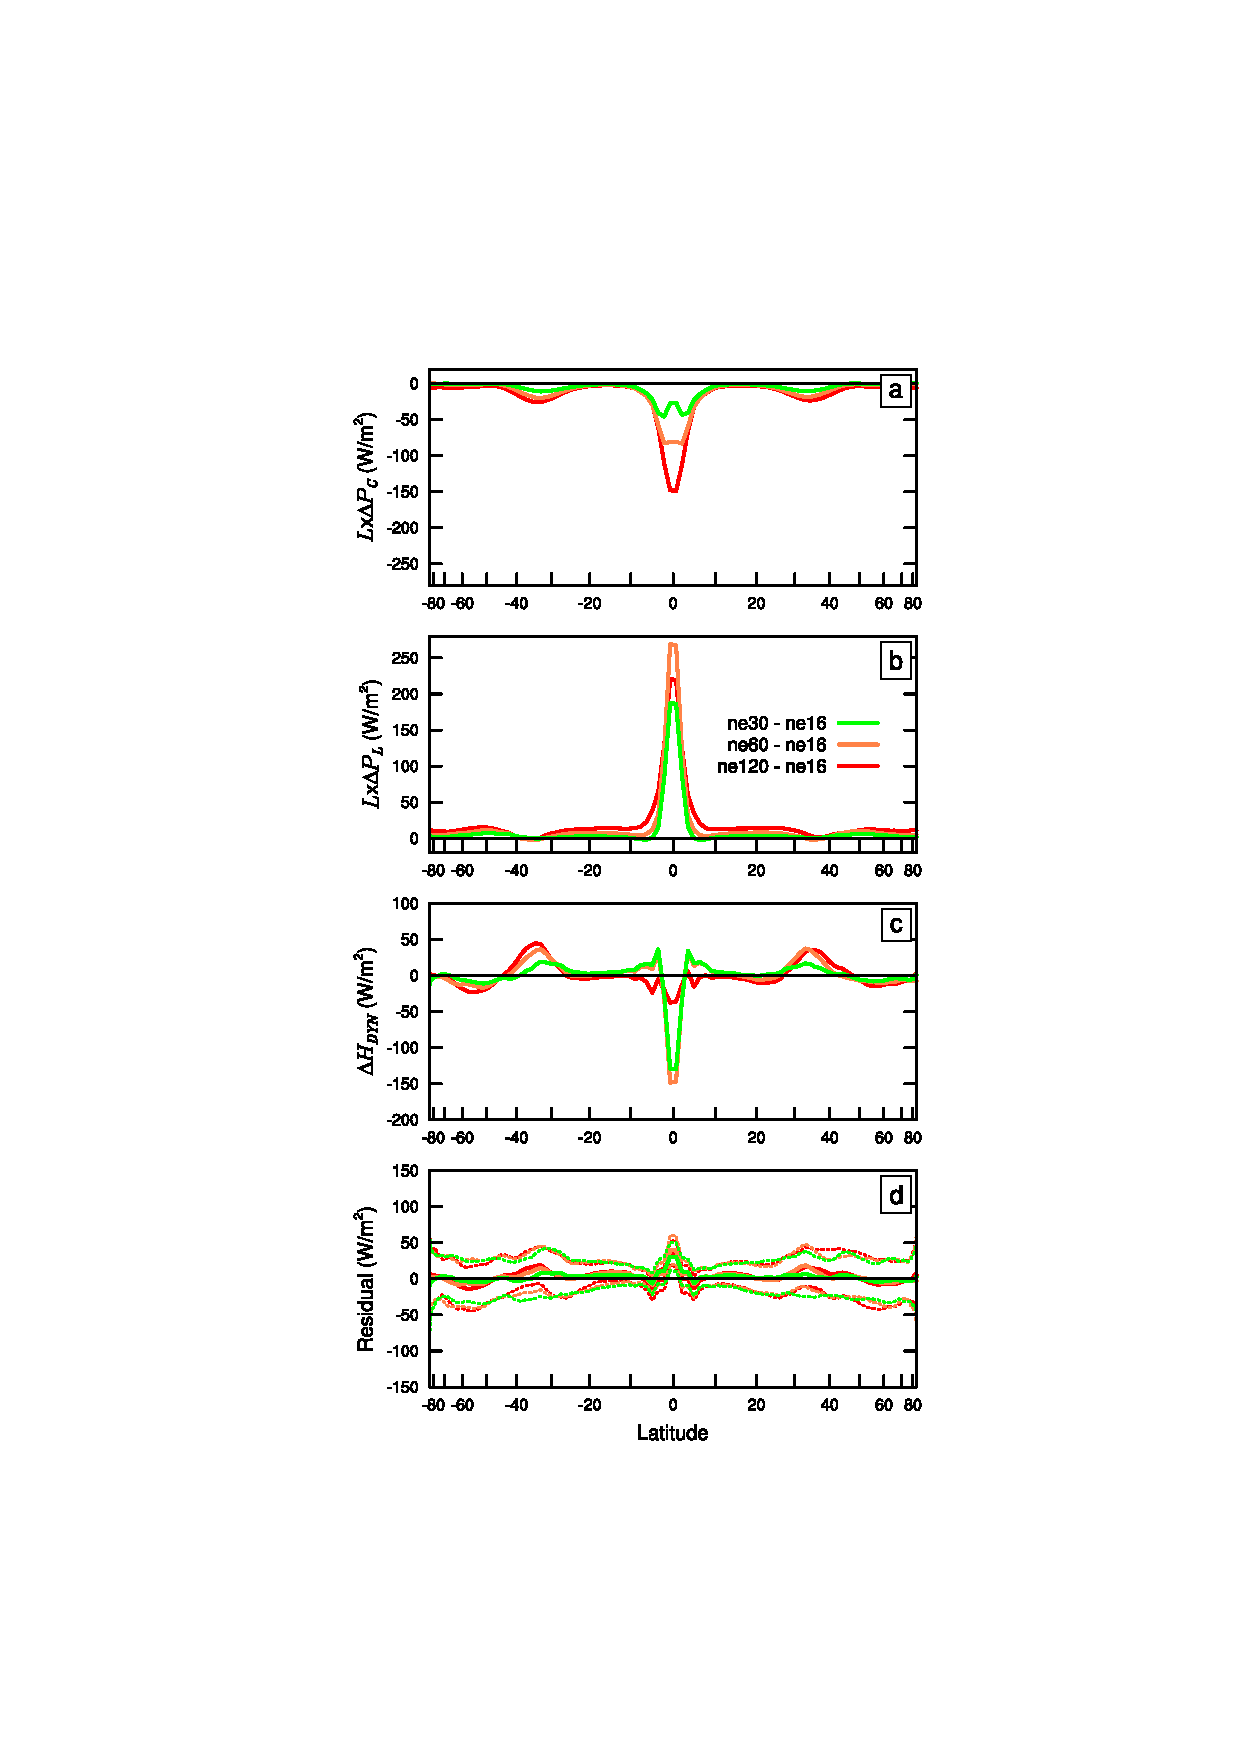
\includegraphics[width=20pc,angle=0]{chapter2/figure1.pdf}\\
\end{center}
\caption{Departure of the components of the zonal average energy budget from the ne16 simulation. Anomalies in latent heat associated with (a) convective precipitation and (b) large-scale precipitation, (c) the dynamical component of the anomalous divergence of the flux of dry static energy by the mean vertical circulation and (d) the residual computed from the sum of (a), (b) and (c). Dotted lines refer to twice the standard deviation associated with low frequency (monthly) variability.}
\label{fig:figure2-1}
\end{figure}

Through evaluating the response of CMIP3 models to global warming emission scenarios, \cite{MO2011NATUREC} have shown that regional changes to the zonal average energy budget are well approximated by the change in the column integrated divergence of the flux of $s$ by the mean vertical circulation, $\Delta H_m$. This term can be decomposed into dynamic, $\Delta H_{DYN}$, and thermodynamic components, $\Delta H_{THM}$, as,
\begin{eqnarray}
\Delta H_m = \Delta H_{DYN} + \Delta H_{THM} = \int \Delta (\overline{\omega}) \frac{d \overline{s}}{dp} + \int \overline{\omega} \Delta (\frac{d \overline{s}}{dp}), \label{eq:eq2-4}
\end{eqnarray}
Making the assumption $\Delta H  \sim \Delta H_m$, the change in the zonally averaged atmospheric energy budget between two simulations may be expressed as,
\begin{eqnarray}
\Delta F_{TOT} (\phi)= L[\Delta P_L (\phi) + \Delta P_C (\phi)] + F_{DC} (\phi) + \Delta H_{DYN} (\phi) + \Delta H_{THM} (\phi), \label{eq:eq2-5}
\end{eqnarray}
where $F_{DC} = F_S + F_{CL} + F_{CD} + F_{SH}$ contains the diabatic cooling terms. Figure~\ref{fig:figure2-1}a,b shows the zonal average latent heat anomalies associated with changes in convective and large-scale precipitation relative to the ne16 simulation. The overall reduction in convective precipitation manifests as a strong, monotonic reduction in latent heating with resolution at the equator, and to a lesser extent in the subtropics. The large-scale precipitation more than compensates for the relative loss of energy due to reductions in convective precipitation at the equator. The anomalous heating due to changes in large-scale precipitation in the ne120 simulation is intermediate to the ne30 and ne60 anomalies at the equator. While the maximum anomalies at the equator are not monotonic with resolution, the width of the equatorial anomaly does become progressively wider with resolution and there is a slight increase in heating with resolution almost everywhere outside the equator.

Figure~\ref{fig:figure2-1}c shows the dynamical component, $\Delta H_{DYN}$ of the divergence of the flux of $s$, due to the change in the mean vertical circulation. The value of $\Delta H_{DYN}$ becomes progressively more negative at the equator in the ne30 and ne60 simulations, and positive anomalies persist just outside the equator. In contrast, the ne120 simulation remains negative just outside the equator and the magnitude of the equatorial minimum in $\Delta H_{DYN}$ is less than in the ne30 or ne60 simulations. Near the subtropics $\Delta H_{DYN}$ becomes increasingly positive with resolution (Figure~\ref{fig:figure2-1}c), indicating enhanced subsidence. Anomalous heating from greater subsiding motion is primarily balanced by reductions in subtropical convective precipitation (Figure~\ref{fig:figure2-1}).

Qualitatively, the spatial distributions of latent heat anomalies are of a similar order of magnitude as $\Delta H_{DYN}$ and appear compensatory. Figure~\ref{fig:figure2-1}d shows the sum of the three terms $L(\Delta P_L + \Delta P_C) + \Delta H_{DYN}$, which may be interpreted as the latent heating anomalies that are not balanced by $\Delta H_{DYN}$. The sum of these three terms is generally small compared to the individual terms, suggestive of a first-order balance of the anomalous energy. 

The relative change in diabatic cooling, $\Delta F_{DC}$, although important in the global mean (Table~\ref{tbl:table2-2}), has very little influence on large regional changes to the energy budget observed in the simulations (not shown). This result is consistent with the response of CMIP3 models to global warming emissions scenarios (Muller an O’Gorman 2011). In contrast to \cite{MO2011NATUREC}, $\Delta H_{THM}$ is also small and shows minimal variation with latitude (not shown). The small contribution of $\Delta H_{THM}$ to the anomalous energy budget indicates that the distribution of $s$ in the simulations is not very sensitive to resolution, partially a reflection of the fixed sea surface temperatures in the aqua-planet configuration. The remaining heating anomalies in Figure~\ref{fig:figure2-1}d may be balanced by neglected transport terms or energy storage.

Interestingly, the residual heating appears to converge to a similar zonal distribution by ne30 (Figure~\ref{fig:figure2-1}d). While the source of this residual may be uncertain, it indicates that the sensitivity of the zonal average energy budget to resolution in the ne30, ne60 and ne120 simulations is contained within the latent heating and $\Delta H_{DYN}$ terms. As $\Delta H_{DYN}$ is proportional to the change in the resolved vertical motion, our results indicate that an active vertical velocity field is providing a balance to the large variations in latent heating observed in the model. \cite{YETAL2014JCLIM} come to a similar conclusion through analysis of the moisture budget for extreme precipitation events, which together indicate that important changes to the resolved vertical velocity field are common to the sensitivity of mean and extreme statistics with resolution.

\begin{figure}
\begin{center}
\noindent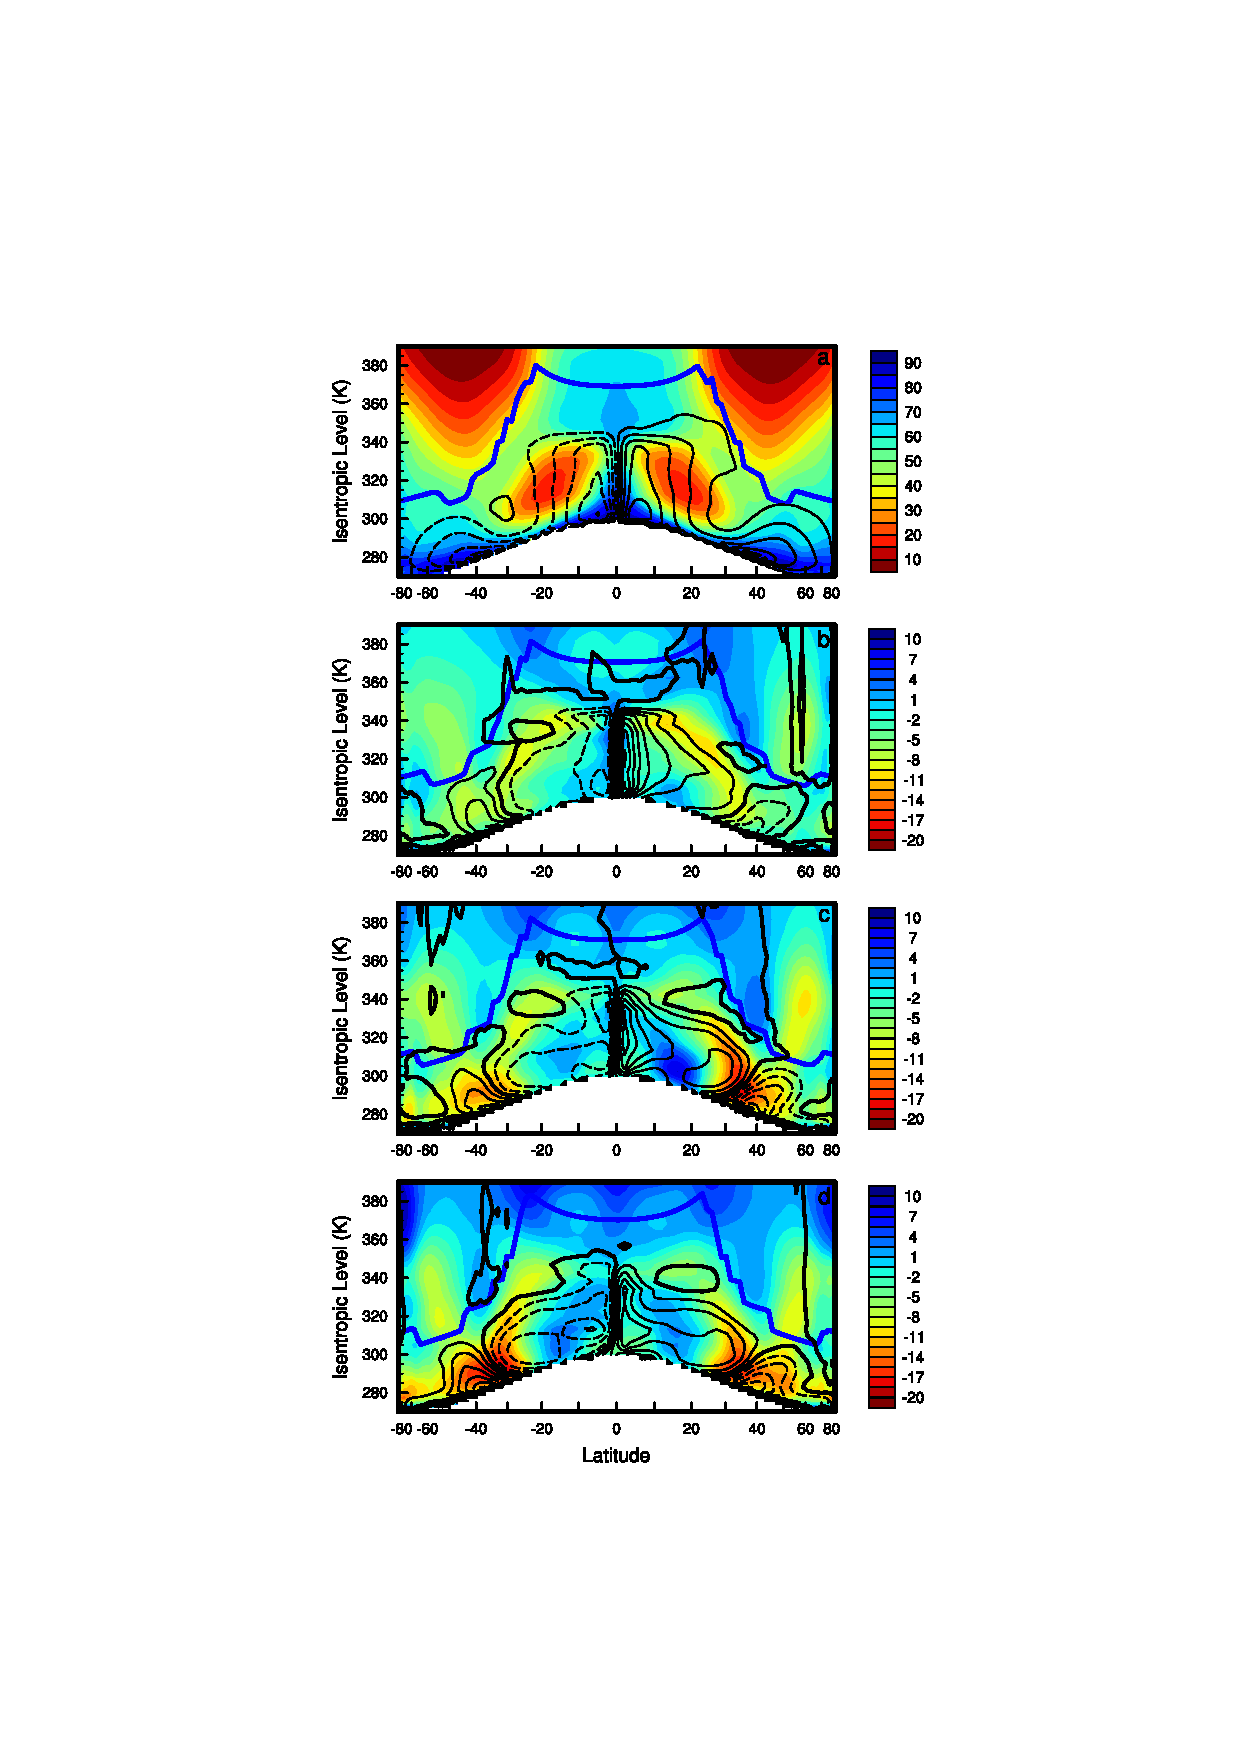
\includegraphics[width=20pc,angle=0]{chapter2/figure2.pdf}\\
\end{center}
\caption{(a) Zonally averaged isentropic meridional streamfunction (black lines) and relative humidity field (color) in the ne16 control. Contour interval is $50 \times 10^9$ kg/s. (b-d) Departures of the zonally averaged isentropic meridional streamfunction and relative humidity field from the ne16 control in the (b) ne30 (c) ne60 and (d) ne120 simulations. Contour interval is $10 \times 10^9$ kg/s. Solid (dashed) lines correspond to clockwise (counter-clockwise) motion and thick solid line corresponds to the zero contour. Blue solid line is the tropopause height computed using a lapse-rate WMO definition.}
\label{fig:figure2-2}
\end{figure}

Changes to the zonal-mean time-mean resolved upward motion near the equator, along with increases in subtropical subsidence, implies a change in the large-scale Hadley Circulation with resolution. Figure~\ref{fig:figure2-2}b-d shows the departure of the mean isentropic meridional mass streamfunction in the simulations from the mean in the control simulation (Figure~\ref{fig:figure2-2}a). At the equator, an anomalous overturning cell extending into the upper-troposphere occurs in the ne30 simulation (Figure~\ref{fig:figure2-2}b). The descending branch of the anomalous equatorial circulation is split between a local branch, confined to within $10^{\circ}$ of the equator, and a poleward traveling branch, flowing under subtropical jet core (not shown) and extending to about $40^{\circ}$ latitude (Figure~\ref{fig:figure2-2}b). The anomalous poleward branch is unique in the sense that the mean Hadley Cell only extends to the latitude of the subtropical jet (Figure~\ref{fig:figure2-2}a), which remains in a fixed location in the simulations \citep{LETAL2015JCLIM}. At higher resolutions, the local descending branch becomes weaker and more confined in the meridional direction, while the poleward branch becomes more pronounced, merging with anomalous upward motion around $20^{\circ}$ to form a partially closed anomalous circulation extending to $40^{\circ}$ latitude (Figures~\ref{fig:figure2-2}c,d). The anomalous ascent near $20^{\circ}$ is consistent with the anomalous off equatorial heating in Figure~\ref{fig:figure2-1}b. While generally the Hadley Cell tends to intensify with resolution, the spatial complexities of the anomalies indicate that changes in the Hadley Cell are not a simple uniform increase in intensity of the mean overturning cell depicted in Figure~\ref{fig:figure2-2}a.

\subsubsection{Moisture Budget}
Changes in the distribution and strength of resolved mass transport in the atmosphere have profound impacts on the distribution of water vapor, which directly influences the cloud amount diagnosed by CAM. Figure~\ref{fig:figure2-2}b-d shows variations in zonal mean relative humidity relative to the ne16 simulation (Figure~\ref{fig:figure2-2}a). Despite increases in relative humidity in and above the upper-troposphere, and within the subtropical dry zone, there is a clear tendency towards a drier atmosphere with resolution. The reduction in global average cloud fraction with resolution (Table~\ref{tbl:table2-1}) is directly related to the reductions in relative humidity, since the macrophysics scheme computes the cloud fraction as a simple function of the relative humidity field in CAM4 \citep{CAM4,PETAL2014JCLIM}. The greatest reduction in clouds occurs at the overlap between where clouds are abundant and regions that experience the greatest amount of drying (not shown).

The most pronounced changes in moisture in the simulations are the progressive reductions in subtropical relative humidity with resolution in the region of elevated subsidence identified in Figure~\ref{fig:figure2-1}c. The maximum reduction in relative humidity occurs in the ne120 simulation, decreasing by a third or 20\% at the 290 K level in the vicinity of $30^{\circ}$ latitude and leading to the complete elimination of clouds in this region (not shown). The drying anomalies are aligned with the anomalous poleward branch, which descends into the region of maximum drying (Figures~\ref{fig:figure2-2}b-d). Drying anomalies also coincide with an anomalous extra-tropical circulation, aligned with an equator-ward subsiding branch that becomes stronger with increasing resolution (Figure~\ref{fig:figure2-2}b-d).

To unravel the role of different processes influencing the relative humidity changes, Figure~\ref{fig:figure2-3} shows some components of the time-mean zonal averaged moisture budget in isentropic coordinates after \cite{SETAL2006JCLIM}, for the northern hemisphere only. The isentropic moisture budget naturally separates along and cross-isentropic mixing, which approximate different mechanisms controlling the relative humidity of the atmosphere \citep{SETAL2006JCLIM}. The descending branch of the Hadley Cell is a cross-isentropic process that exports dry air from upper levels to lower levels of the troposphere \citep{P1999GM}. The moisture budget of the subtropics is also influenced by extra-tropical recirculation, which is an approximately adiabatic process \citep{GETAL2005JAS,SETAL2006JCLIM}. Extra-tropical recirculation refers to moisture advected out of the subtropics, condensing along poleward trajectories and re-circulating back into the subtropics \citep{GETAL2005JAS}.

The zonal averaged moisture balance in isentropic coordinates is \citep{SETAL2006JCLIM},
\begin{eqnarray}
\partial_t (\overline{\rho_{\theta}} \, \overline{q}^{\ast}) + \partial_y (\overline{\rho_{\theta}} \, \overline{v}^{\ast} \, \overline{q}^{\ast}) + \partial_{\theta} (\overline{\rho_{\theta}} \overline{Q}^{\ast} \overline{q}^{\ast}) + \partial_y (\overline{\rho_{\theta}} \, \overline{v^{\prime} q^{\prime}}) + \partial_{\theta} (\overline{\rho_{\theta}} \, \overline{Q^{\prime} q^{\prime}}) = \overline{\rho_{\theta}} \overline{S}^{\ast}, \label{eq:eq2-6}
\end{eqnarray}
where $q$ is the specific humidity, $S = \frac{dq}{dt}$ and $Q = \frac{d \theta}{dt}$ are the specific humidity and diabatic forcing terms from the column physics. Primes denote fluctuations about the zonal and temporally averaged mean. The zonal average moisture tendency in isentropic coordinates reflects a balance between moisture sources, $\overline{\rho_{\theta}} \overline{S}^{\ast}$, and the divergence of mean and eddy fluxes of moisture along and across isentropic surfaces.

\begin{figure}
\begin{center}
\noindent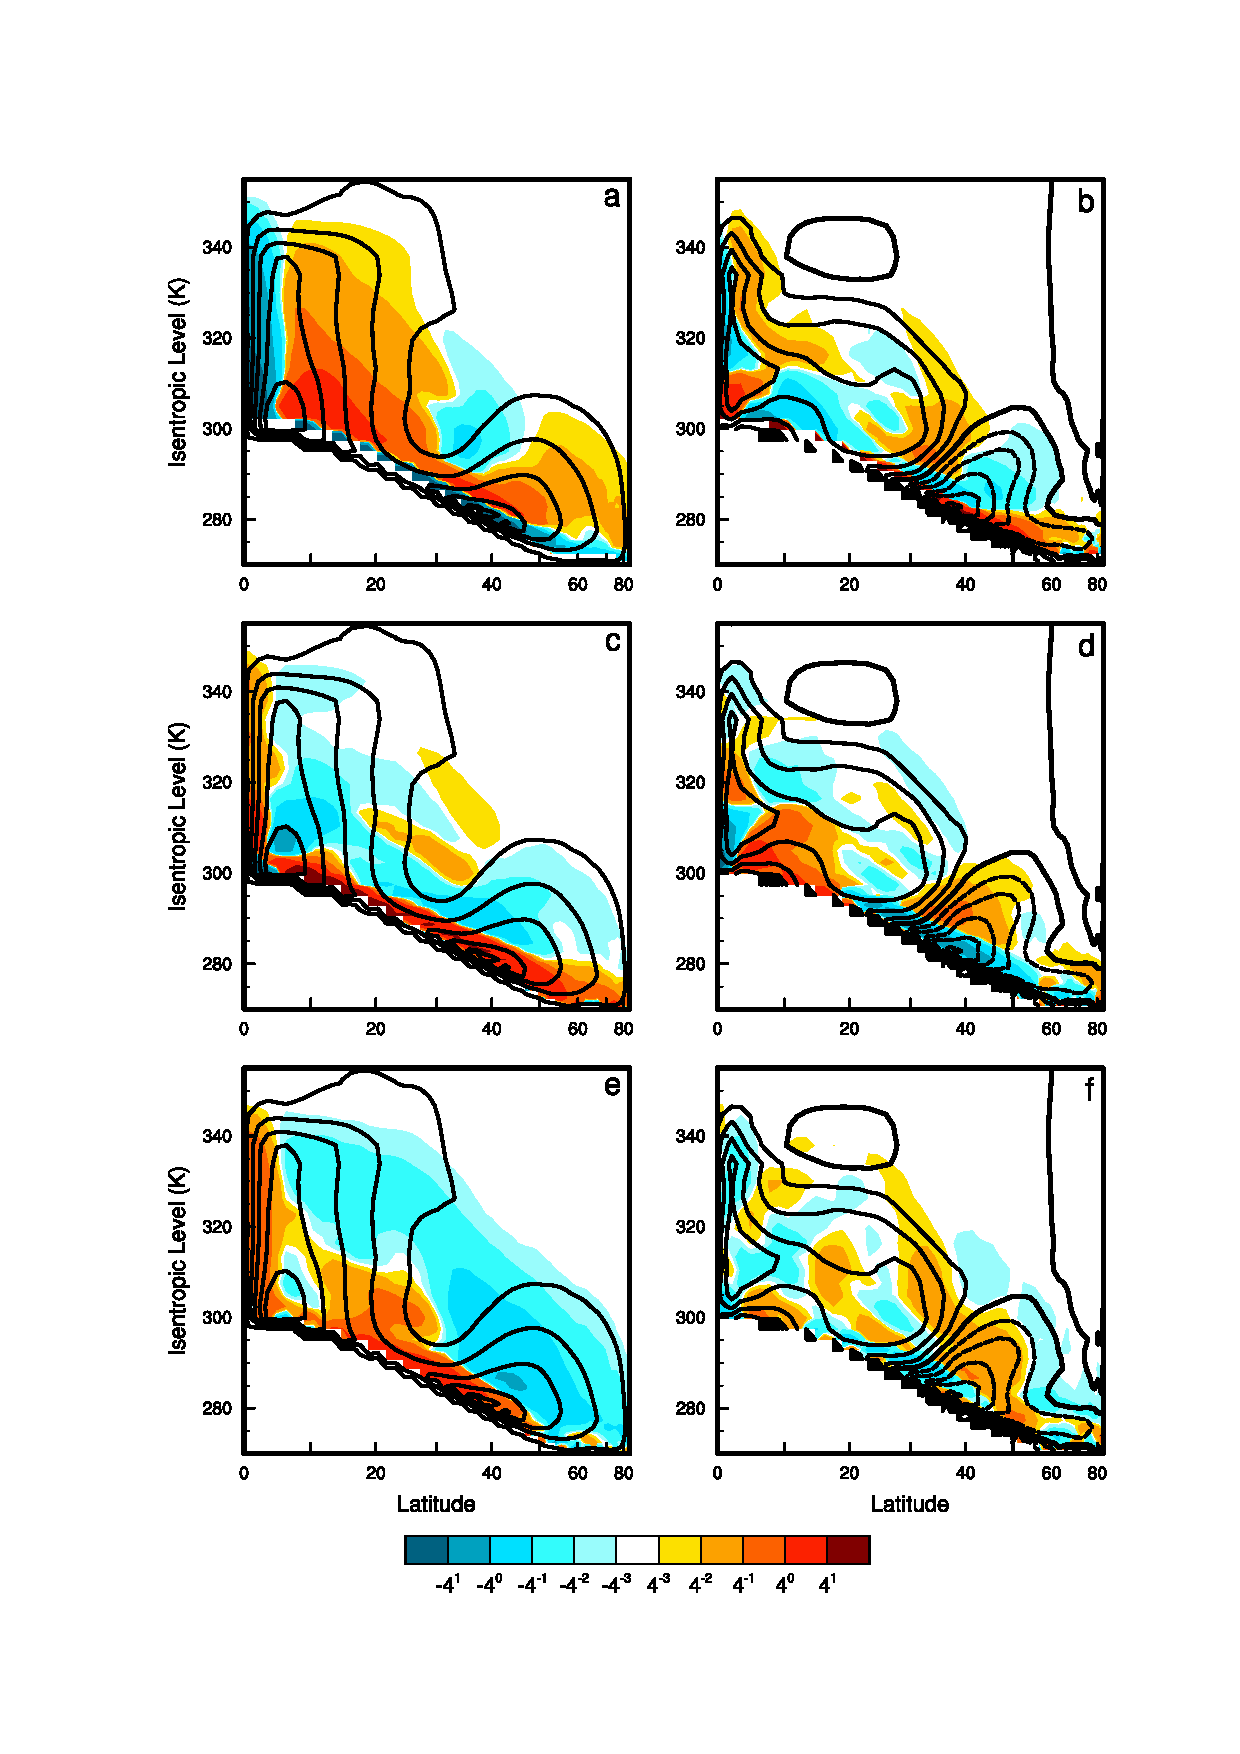
\includegraphics[width=30pc,angle=0]{chapter2/figure3.pdf}\\
\end{center}
\caption{(a), (c) and (e) Components of the zonal average moisture budget in isentropic coordinates in the ne30 simulation. (b), (d) and (e) Departure of the components of the zonally averaged moisture budget in the ne120 simulation from the ne16 control. (a), (b) Divergence of the cross isentropic moisture transport by the mean, (c), (d) divergence of the along isentropic moisture transport by the mean and (e), (f) divergence of the along isentropic eddy transport. Units are in $10^{-6}$ kg/m2/K/s and the meridional streamfunction contours are as in Figure~\ref{fig:figure2-2}.}
\label{fig:figure2-3}
\end{figure}

Figure~\ref{fig:figure2-3}b,d,f show the departure of the mean cross-isentrope, $\partial_{\theta} (\overline{\rho_{\theta}} \overline{Q}^{\ast} \overline{q}^{\ast})$, mean along-isentrope, $\partial_y (\overline{\rho_{\theta}} \, \overline{v}^{\ast} \, \overline{q}^{\ast})$, and eddy along-isentrope, $\partial_y (\overline{\rho_{\theta}} \, \overline{v^{\prime} q^{\prime}})$, terms in the ne120 simulation relative to the ne16 simulation values, given in Figure~\ref{fig:figure2-3}a,c,e. The remaining terms of moisture budget could not be computed directly from the available model output. Anomalies in the mean cross-isentropic flux of moisture near the equator are characterized by low-level divergence and convergence aloft (Figure~\ref{fig:figure2-3}b). This pattern indicates extraction of moisture from the lower troposphere into the middle troposphere due to greater equatorial ascent. Anomalies in along-isentropic fluxes (Figure~\ref{fig:figure2-3}d,f) supply the lower troposphere with moisture at the equator, maintaining the cross-isentropic anomalies.

The large subtropical drying anomaly near $40^{\circ}$ (Figure~\ref{fig:figure2-2}d) is supported by anomalous divergence from all terms shown in Figure~\ref{fig:figure2-3}. The reduction in convective precipitation near $40^{\circ}$ opposes drying through relative increases in moisture source (not shown). The divergence of along isentropic eddy fluxes (Figure~\ref{fig:figure2-3}c) is most closely aligned with the drying anomaly flanking the anomalous poleward flow and extending into the region of maximum drying near $40^{\circ}$ (Figure~\ref{fig:figure2-2}d). This result is suggestive of greater eddy activity along the anomalous poleward flow. Figure~\ref{fig:figure2-4} shows the changes in the eddy momentum fluxes, $\overline{u^{\prime} v^{\prime}}$, with resolution, relative to the eddy fluxes in the ne16 simulation (Figure~\ref{fig:figure2-4}a). An increase in eddy activity lies just above the anomalous poleward flow, and the magnitude of the anomalous eddy fluxes increase with resolution (Figure~\ref{fig:figure2-4}). Alignment of the anomalous poleward flow with the anomalous eddy fluxes is suggestive of a momentum balance between the Coriolis force and the divergence of the eddy fluxes. Alternatively, the increased wave activity may be related to a reduction in effective dissipation of potential vorticity with resolution \citep{LETAL2015JCLIM}. 

\begin{figure}
\begin{center}
\noindent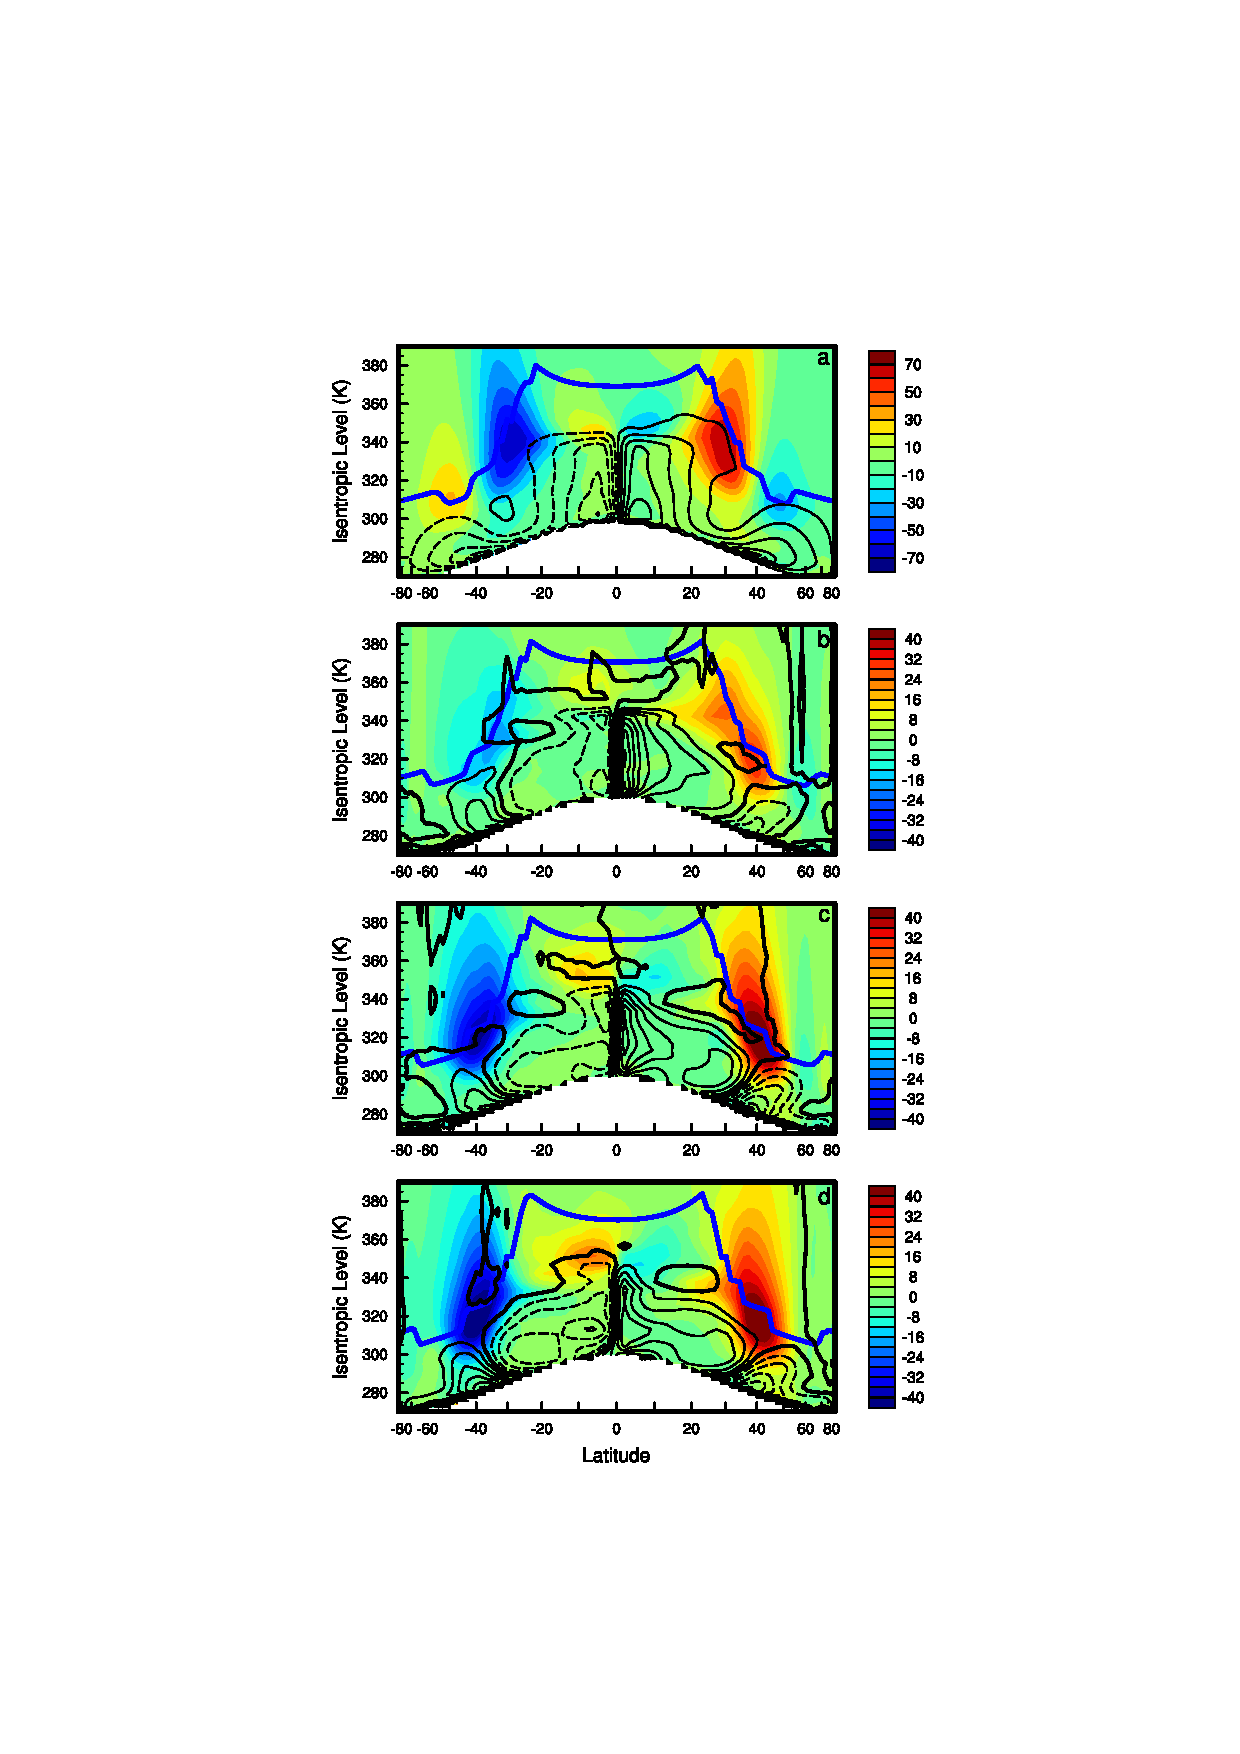
\includegraphics[width=20pc,angle=0]{chapter2/figure4.pdf}\\
\end{center}
\caption{As in Figure~\ref{fig:figure2-2}, but for the eddy fluxes $\overline{u^{\prime} v^{\prime}}$ in units of m2/s2.}
\label{fig:figure2-4}
\end{figure}

The large changes in cloud fraction (Table~\ref{tbl:table2-1}) are balanced by greater overturning of the Hadley Cell, greater isentropic mixing associated with variations in the extra-tropical circulation and a reduction in activity of the convection scheme. While this is not a particularly new finding \citep{KW1991JGR}, it indicates that the same underlying sensitivity of cloud coverage to resolution has continued to persist within the CAM lineage for at least 25 years.

\subsection{An Explanation}
Our results have demonstrated that a progressive drying of the atmosphere with increasing resolution is balanced through tropical and extra-tropical changes to the large-scale circulation. Here, we make the important simplification that many of the complexities embedded in the sensitivity of the large-scale circulation to horizontal resolution is a non-linear response to a resolution sensitive process rooted in linear Boussinesq theory. This simplification is unverified - its purpose is to provide the simplest possible interpretation of the resolution signal that is consistent with linear theory. We recognize that there may be other important resolution sensitive processes \citep[e.g.,][]{LETAL2015JCLIM}, but suggest that they are not sufficient to explain the large changes to the hydrologic cycle identified in the simulations. 

We begin with a non-hydrostatic, dry, non-rotating, frictionless atmosphere with no heat sources, a framework often used in the analysis of internal gravity waves \citep{H2004}. While the neglect of moist processes is clearly invalid for a moist GCM, the simplified framework may be viewed as approximating the evolution of individual dynamics time-steps in response to buoyant perturbations passed from the column physics. For solutions to a linearized vertical velocity perturbation of the type $w = w_0 exp[i(kx + mz + \sigma t)]$ in an unstable atmosphere, let $X^2 = -| N^2 |$, where $N^2$ is the buoyancy frequency. The dispersion relation is, 
\begin{eqnarray}
\sigma^2 = X^2 \frac{k^2}{k^2 + m^2},\label{eq:eq2-7}
\end{eqnarray}
where $\sigma$ is the unstable growth rate, $k$ is the horizontal wavenumber and $m$, the vertical wavenumber. According to equation~\ref{eq:eq2-7}, the growth rate is bounded by $X$ since $k/\sqrt{k^2 + m^2}$ is bounded by unity. That is, convergence occurs as the horizontal scale of motion is reduced from the hydrostatic limit ($k \ll m$), to within the non-hydrostatic limit ($k \approx m$). For deep tropospheric perturbations, the non-hydrostatic limit occurs at horizontal resolutions approaching the depth of the troposphere.

At hydrostatic scales ($k \ll m$), the unstable growth rate is approximately linear in $k$ (equation~\ref{eq:eq2-7}). The significance of $k$ in the numerator of equation~\ref{eq:eq2-7} can be traced back to the horizontal scale of the locally balanced hydrostatic pressure perturbation \citep{JR2016QJRMS}, driving horizontal convergence into the unstable air column and vertical motion. A model that permits removal of convective instability by the resolved dynamics results in an unstable growth rate, $\sigma$, that is linear in $k$ at hydrostatic scales. This result is true of both hydrostatic and non-hydrostatic models. The equivalent dispersion relation for hydrostatic models is $\sigma^2 = X^2 (k^2 / m^2)$, implying that hydrostatic solutions are unbounded in scale in the non-hydrostatic regime \citep{O1981JAS}, referred to as an ``ultra-violet catastrophe." This ultra-violet catastrophe is not relevant at typical truncation scales of present day GCMs. 

We hypothesize that the horizontal scale of the diabatic forcing from the column physics is proportional to the grid spacing, decreasing the horizontal scale of the hydrostatic pressure perturbations and increasing the unstable growth rate $\sigma$ and resolved vertical motion as the resolution is increased. A reduction in horizontal scale of the diabatic forcing arising from the column physics was identified in CAM by \cite{HETAL2006JCLIM}. Our hypothesis was motivated in part by the study of \cite{W1999T}, where convergence of the Hadley Cell was recovered in a prior version of CAM through fixing the horizontal scale of the physics forcing and increasing the resolution of the dynamical core. Our hypothesis attempts to explain the sensitivity of the resolved vertical motion in CAM with resolution identified in this study, and others \citep{KW1991JGR,LETAL2011TELLUS,YETAL2014JCLIM,OETAL2016JAMES}.

\begin{table}[t]
\begin{center}
\noindent\includegraphics[width=20pc,angle=0]{chapter2/table3.pdf}\\
\end{center}
\caption{Mean upward vertical pressure velocity at 600 hPa and the fraction of time the deep convection scheme is active in the simulations (FREQZM) in the region $10^{\circ}$ N to $10^{\circ}$ S. }
\label{tbl:table2-3}
\end{table}

Mean values of the vertical pressure velocity at the 600 hPa level, conditionally sampled for upward motion in the ascent region of the Hadley Cell ($10^{\circ}$ N to $10^{\circ}$ S) are shown in Table~\ref{tbl:table2-3}. No interpolation was performed during this calculation and all values were computed on their native grids. Ascent velocities associated with the Hadley Cell increase with resolution, and show no indication of convergence. 

We argue that the increases in mean vertical velocities in Table~\ref{tbl:table2-3} are due to contributions of increasingly finer scales with increasing horizontal resolution. Figure~\ref{fig:figure2-5} shows the power spectra of 600 hPa vertical pressure velocities over the entire domain in the simulations, including upward and downward motion. Wavenumbers on the order 10 or less appear converged, potentially reflecting the ability of the model to resolve the deformation radius in all simulations and enabling realistic interactions between mid-latitude eddies and the mean flow \citep{W1999T,DV2000JCLIM,ZGETAL2015JAMES}. For wavenumbers on the order of 10 or larger, the general trend is for reduced power at lower wavenumbers and increased power at higher wavenumbers with increasing resolution (Figure~\ref{fig:figure2-5}). 

Snapshots of the vertical pressure velocities at the equator for the four different resolutions (Figure~\ref{fig:figure2-6}) provide further evidence that a transfer of variance to finer scales contributes to the observed variations in the mean state (Table~\ref{tbl:table2-3}). Resolved convective updrafts populate the equator, and their horizontal scale decreases with increasing resolution. This transfer of velocity variance to finer scales is consistent with the model results and emergent scaling presented by \cite{RETAL2016CD}, as well as linear Boussinesq theory (equation~\ref{eq:eq2-7}).

\begin{figure}[t]
\begin{center}
\noindent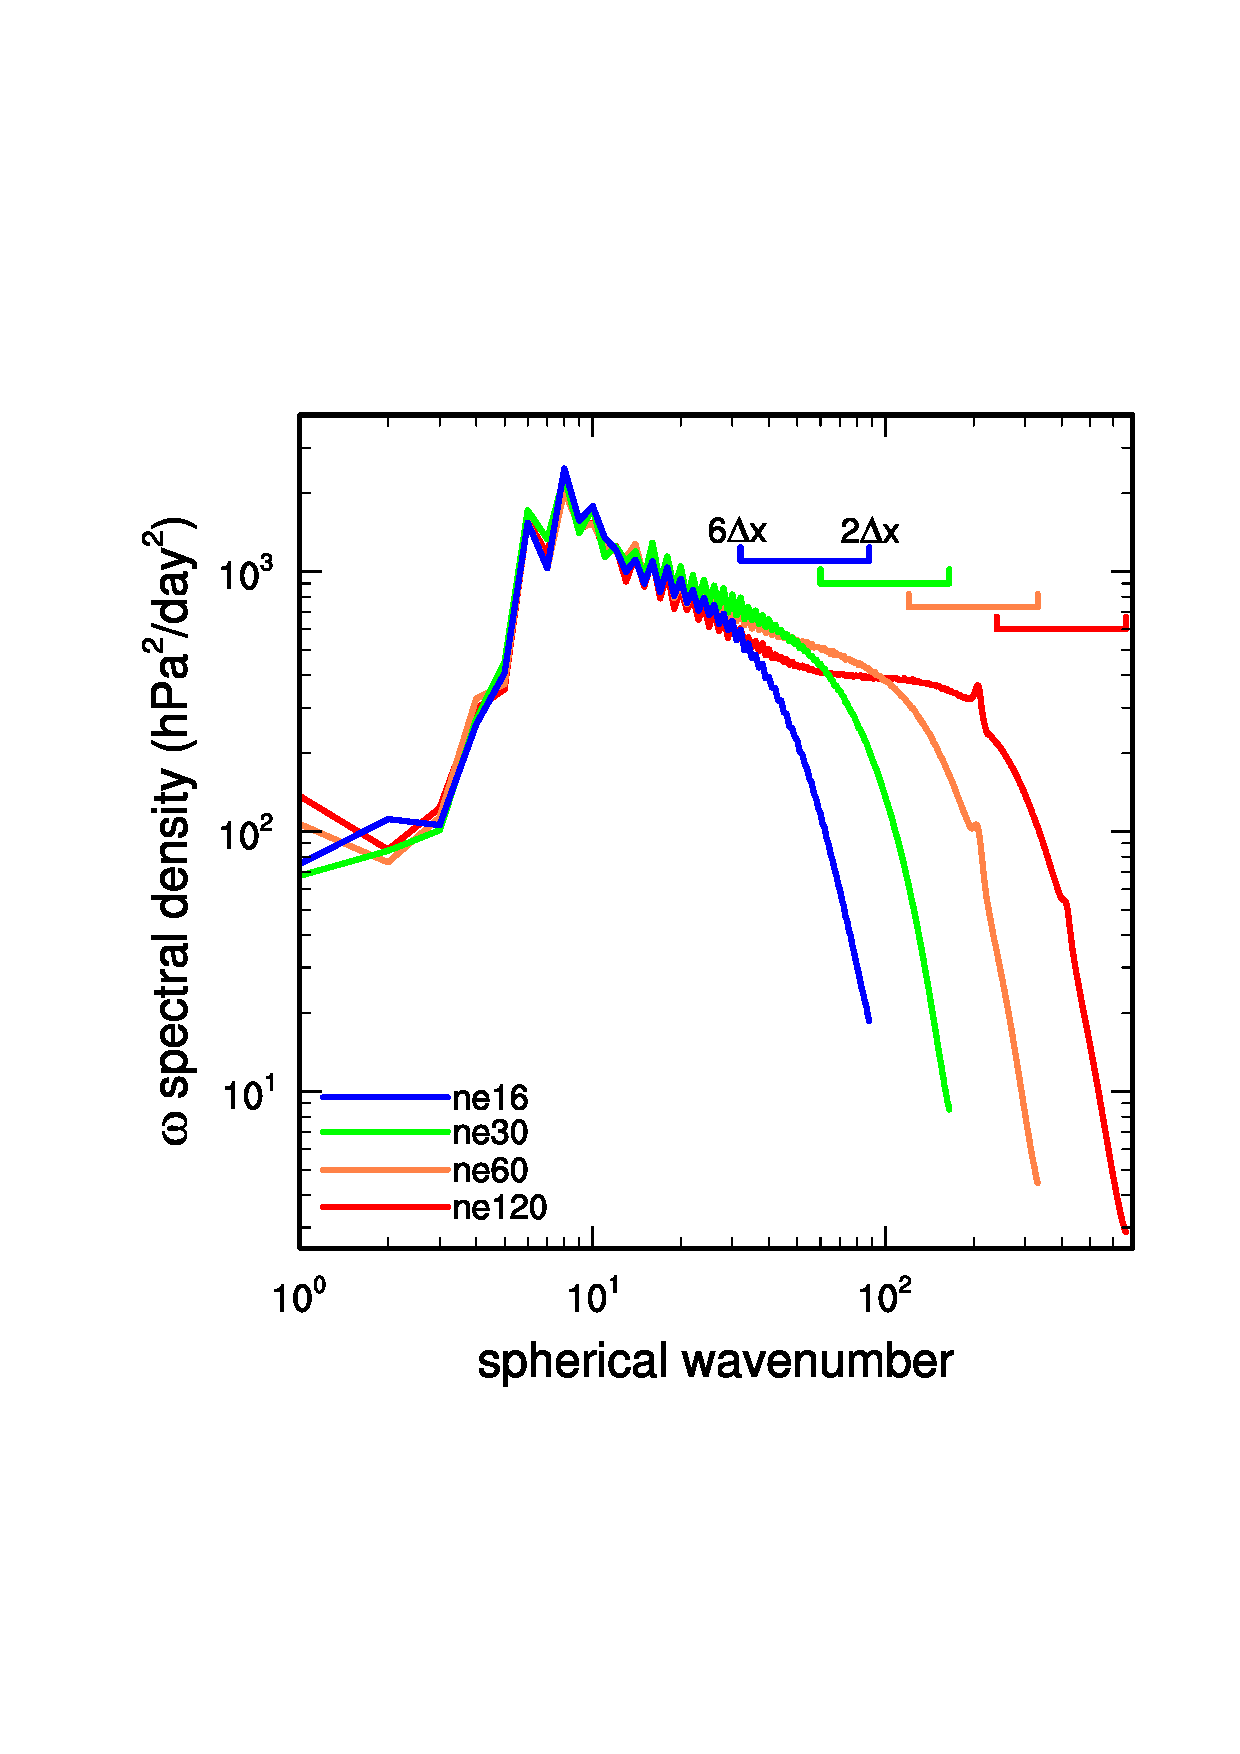
\includegraphics[width=20pc,angle=0]{chapter2/figure5.pdf}\\
\end{center}
\caption{Power spectral density of the 600 hPa vertical pressure velocity over the entire model domain. Values computed from 360 instances of 6-hourly output randomly selected from the integration period.}
\label{fig:figure2-5}
\end{figure}

\begin{figure}
\begin{center}
\noindent\includegraphics[width=35pc,angle=0]{chapter2/figure6.pdf}\\
\end{center}
\caption{Longitude-height instantaneous snapshot of the vertical pressure velocity at the equator during a randomly chosen time in the (a) ne16 (b) ne30 (c) ne60 and (d) ne120 simulations.}
\label{fig:figure2-6}
\end{figure}

The linear theory, and our hypothesis in general, is only applicable to convectively unstable conditions within the dynamical core. The occurrence of convectively unstable conditions may be thought to be infrequent in GCMs, as the convection schemes are designed to prevent the occurrence of resolved convection. Figure~\ref{fig:figure2-6}, however, provides evidence that resolved convection is a common occurrence in the deep tropics in CAM. Here, we propose an explanation for the occurrence of resolved convection in the presence of a convection scheme in CAM. The relevant ordering of the sub-models in our simulations, on the level of an individual physics time-step is the convection schemes, the large-scale precipitation scheme and the dynamics, respectively \citep{CAM4}. This process ordering implies that convectively unstable air produced by the large-scale condensation scheme interacts directly with the dynamics before the convection schemes are able to consume the instability. The resolved dynamics consume buoyancy at a rate proportional to $\omega$ in the thermodynamic equation, whose dynamics are approximated by the dispersion relation (equation~\ref{eq:eq2-7}). As the horizontal resolution of the model increases, resolved updrafts intensify with resolution, consuming buoyancy at an increasing rate. The convection scheme is then left with a smaller proportion of the available potential energy initially produced through the large-scale precipitation scheme. A caveat to this explanation is that the mean state is determined by the solution trajectory spanning many time-steps, which may not be reflective of processes occurring in a single time-step.

The activity of the deep convection scheme in the model is tied to an estimate of the available potential energy using a dilute plume calculation after \cite{RB1992JAS}. Although this quantity departs from the usual definition of the convective available potential energy (CAPE), we will refer to this quantity as CAPE throughout the discussion to be consistent with prior CAM studies. When CAPE exceeds 70 J/kg, the deep convection scheme is triggered (Neale et al. 2010). Unfortunately, CAPE is not available from the model output and we do not attempt to diagnose it from the available fields. A related quantity, the fraction of time in which the deep convection scheme is active in the simulations (FREQZM), is available from the model output and the mean values for the deep tropics are provided in Table~\ref{tbl:table2-3}. FREQZM is systematically reduced as the vertical velocities increase with resolution. We speculate that the resolved vertical motion becomes more effective at consuming available potential energy with increasing resolution, thereby reducing the frequency in which CAPE reaches its threshold value of 70 J/kg.

\begin{figure}
\begin{center}
\noindent\includegraphics[width=20pc,angle=0]{chapter2/figure7.pdf}\\
\end{center}
\caption{(a) Probability density distributions of 600 hPa vertical pressure velocity conditionally sampled for upward motion in the region $10^{\circ}$ N to $10^{\circ}$ S. (b) Probability density distribution of vertical pressure velocities in (a) rescaled to the ne120 simulation using a $\Delta x^{-1}$ scaling (solid thin lines) and a $\Delta x^{-2/3}$ scaling (dotted thin lines). Values computed from 1460 instances of 6-hourly output randomly selected from the integration period.}
\label{fig:figure2-7}
\end{figure}

While we don’t expect the steady-state GCM solutions of vertical velocity to be linear in $k$, it is instructive to determine the degree to which the linear scaling reflects the full solution. To perform the scaling, we take the grid spacing, $\Delta x$, from the four simulations and scale the vertical velocities in the ne16, ne30 and ne60 simulations to the scale of the ne120 simulation using a $k \propto \Delta x^{-1}$ scaling. The probability density distribution of resolved upward motion in the deep tropics for all simulations are shown in Figure~\ref{fig:figure2-7}a, and the scaled distributions are provided in Figure~\ref{fig:figure2-7}b. The $\Delta x^{-1}$ relationship does a poor job of explaining the sensitivity of the resolved vertical motion to horizontal resolution, systematically over predicting the vertical velocities compared to the ne120 simulation.

The $\Delta x^{-1}$ scaling is an interpretation of the dispersion relation \citep{WK1982MWR}, but may also be derived from a scale analysis of the kinetic energy budget \citep{PG2006JAS} or the Poisson equation \citep{JR2016QJRMS}. Because of the the poor fit of the $\Delta x^{-1}$ scaling on the model solutions (Figure~\ref{fig:figure2-7}b), it might be tempting to abandon our explanation altogether. However, the physics of the $\Delta x^{-1}$ scaling has a strong theoretical foundation, and instead we reconcile our explanation with a modification. We argue that the linear Boussinesq scaling is reflective of what occurs in GCMs, but that additional processes, likely associated with parameterized moist processes and resulting feedbacks onto the general circulation, steer the solution away from a $\Delta x^{-1}$ scaling. 

\cite{RETAL2016CD} propose a shallower scaling exponent of $\Delta x^{-2/3}$. The  is the scaling that results from applying mass continuity to the $-5/3$  spectral slope of the horizontal winds typical of mesoscale circulations \citep{RETAL2016CD}. For comparison, the $\Delta x^{-2/3}$ scaling is overlain in Figure~\ref{fig:figure2-5}b. While the $\Delta x^{-2/3}$ scaling overestimates the vertical velocities compared to the ne120 simulation, the overestimate is much less than any single curve using the $\Delta x^{-1}$ scaling, and the scaled distributions all line up on top of one another. The \cite{RETAL2016CD} scaling is clearly a more accurate representation of the sensitivity of the fully coupled solution to horizontal resolution than that provided by linear Boussinesq theory.

\subsection{Conclusions}
We have studied the convergence of the mean state of the spectral element version of the Community Atmosphere Model (CAM) coupled to the version 4 physics package in an aqua-planet configuration. As the horizontal resolution is increased, the atmosphere progressively dries, cloud cover decreases and the large-scale precipitation rate increases at the expense of convective precipitation. Variations in the global atmospheric energy budget are primarily a reflection of these changes, resulting in a reduction in longwave cloud forcing and an increase in clear-sky transmissivity with resolution. The regional atmospheric energy budget indicates that large-scale precipitation increases are balanced by anomalous convergence of dry-static energy transport, due to increasing mean vertical velocities in the deep tropics. An analysis of the moisture budget reveals that the drying trend in the simulations is balanced by anomalous divergence of moisture fluxes associated with an intensification of the Hadley Cell and simultaneous changes to the extra-tropical circulation. The large reductions in cloud fraction with resolution are a result of a lower relative humidity field and reductions in activity of the convection scheme. 
 
A possible explanation for the resolution sensitivity of the mean state was formulated, inspired by the experiments of \cite{W1999T} and linear Boussinesq theory. We hypothesize that an increase in horizontal resolution leads to a reduction in horizontal scale of the diabatic forcing from the column physics, facilitating fine-scale flow and faster resolved convective updrafts within the dynamical core. Since buoyancy consumption is proportional to the magnitude of resolved upward motion, the dynamical core becomes more efficient at consuming buoyancy with resolution. As a result of the process ordering within CAM, and presumably other General Circulation Models \citep{B1991ECMWF}, the convection scheme may only remove buoyancy produced through large-scale precipitation after the dynamics have had an opportunity to consume of some of the buoyancy, which we speculate results in a reduction in activity of the convection scheme with resolution.

It is difficult to provide definitive proof of our explanation from an analysis of the aqua-planet experiments. We suggest that the reason for this difficulty is because the implied $\Delta x^{-1}$ dependence of the resolved vertical velocity elicits a non-linear response, pushing the full solution towards a new equilibrium that departs from $\Delta x^{-1}$ scaling. We have developed some simple deterministic dry experiments to test our hypothesis, using idealized diabatic forcing. Our results indicate that a $\Delta x^{-1}$ dependency is a robust feature of the spectral element dynamical core in CAM \citep{HR2018JAMES}. Future work will target how the inclusion of moist parameterizations effects the  scaling.

The strong coupling of the large-scale precipitation scheme with the dynamics at high horizontal resolution, but still within the hydrostatic regime, has been shown to be important for the simulation of Tropical Cyclones \citep{ZHL2012JAS} and precipitation extremes \citep{LETAL2011TELLUS,YETAL2014JCLIM,RETAL2016CD,OETAL2016JAMES}. Our explanation, if confirmed, implies that the interaction of the large-scale precipitation scheme with the dynamics is highly dependent on the horizontal resolution, and efforts to produce ‘scale-aware’ closures may need to focus on this interaction to preserve some of the benefits of high-resolution simulations. 